\documentclass[twocolumn]{aastex631}
\received{\today}
\shorttitle{APO Proposal}
\graphicspath{{figures/}}

\usepackage{lipsum}
\usepackage{physics}
\usepackage{multirow}
\usepackage{xspace}
\usepackage{natbib}
\usepackage{fontawesome5}
\usepackage{xcolor}
\usepackage{wrapfig}
\usepackage[figuresright]{rotating}

% remove indents in footnotes
\usepackage[hang,flushmargin]{footmisc} 

\newcommand{\todo}[1]{{\color{red}{[TODO: #1}]}}
\newcommand{\needcite}{{\color{magenta}{(needs citation)}}}
\newcommand{\placeholder}[1]{{\color{gray} \lipsum[#1]}}

% custom function for adding units
\makeatletter
\newcommand{\unit}[1]{%
    \,\mathrm{#1}\checknextarg}
\newcommand{\checknextarg}{\@ifnextchar\bgroup{\gobblenextarg}{}}
\newcommand{\gobblenextarg}[1]{\,\mathrm{#1}\@ifnextchar\bgroup{\gobblenextarg}{}}
\makeatother

\begin{document}

\title{{\Large Planetary Radius Valley Investigation}\\\vspace{0.15cm}ASTR 581 APO Proposal}

% affiliations
\newcommand{\UW}{Department of Astronomy, University of Washington, Seattle, WA, 98195}

\author[0000-0001-6147-5761]{Tom Wagg}
\affiliation{\UW}

\correspondingauthor{Tom Wagg}
\email{tomwagg@uw.edu}

\section{Introduction}
\placeholder{1-3}

\begin{figure}
    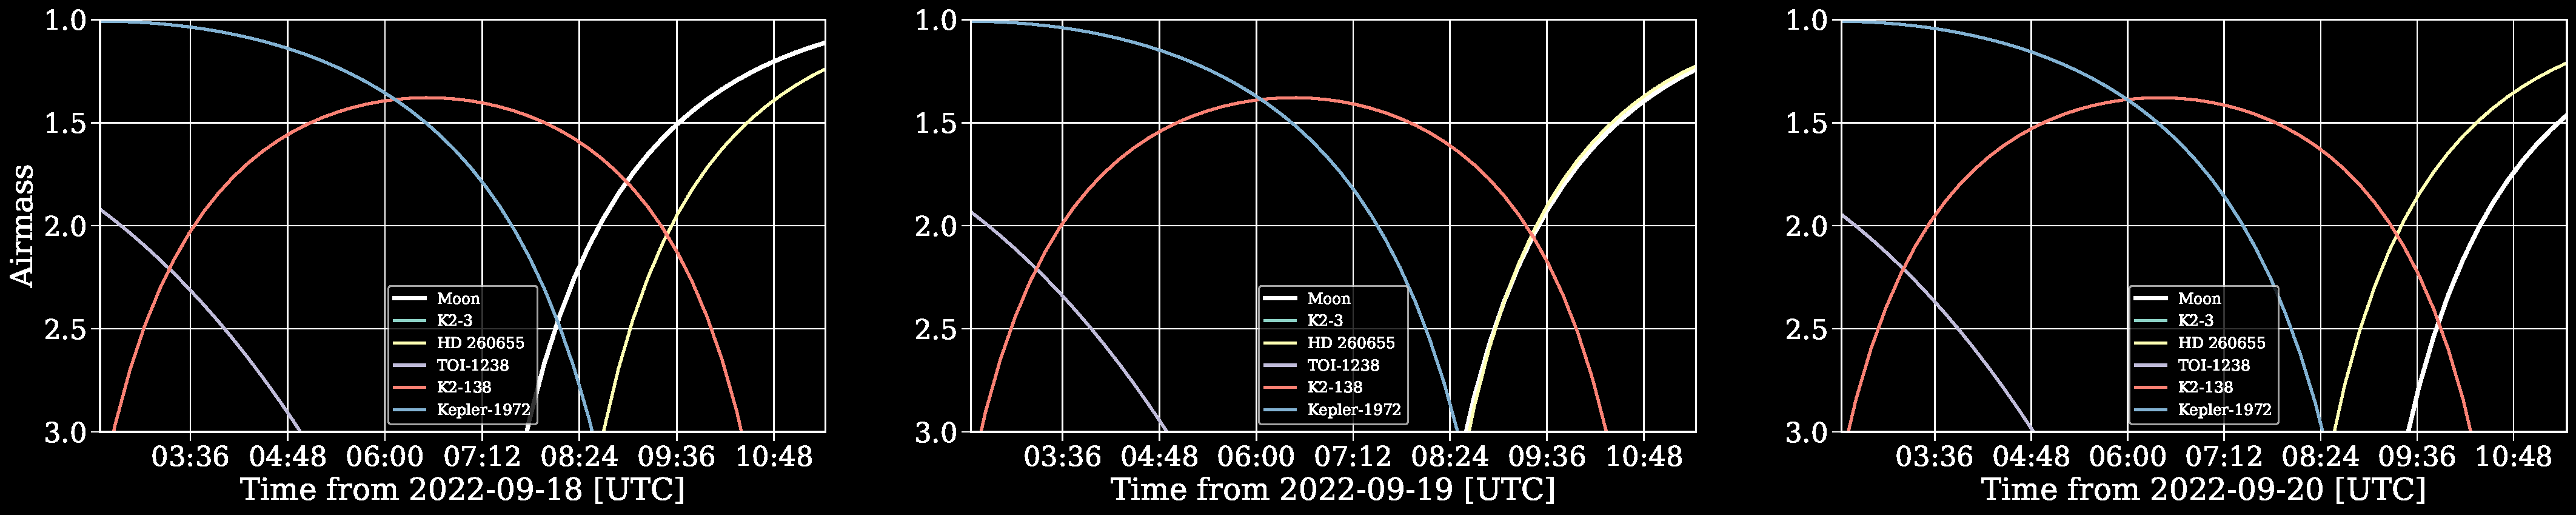
\includegraphics[width=\columnwidth]{potential_systems.pdf}
    \caption{}
\end{figure}

\begin{figure}
    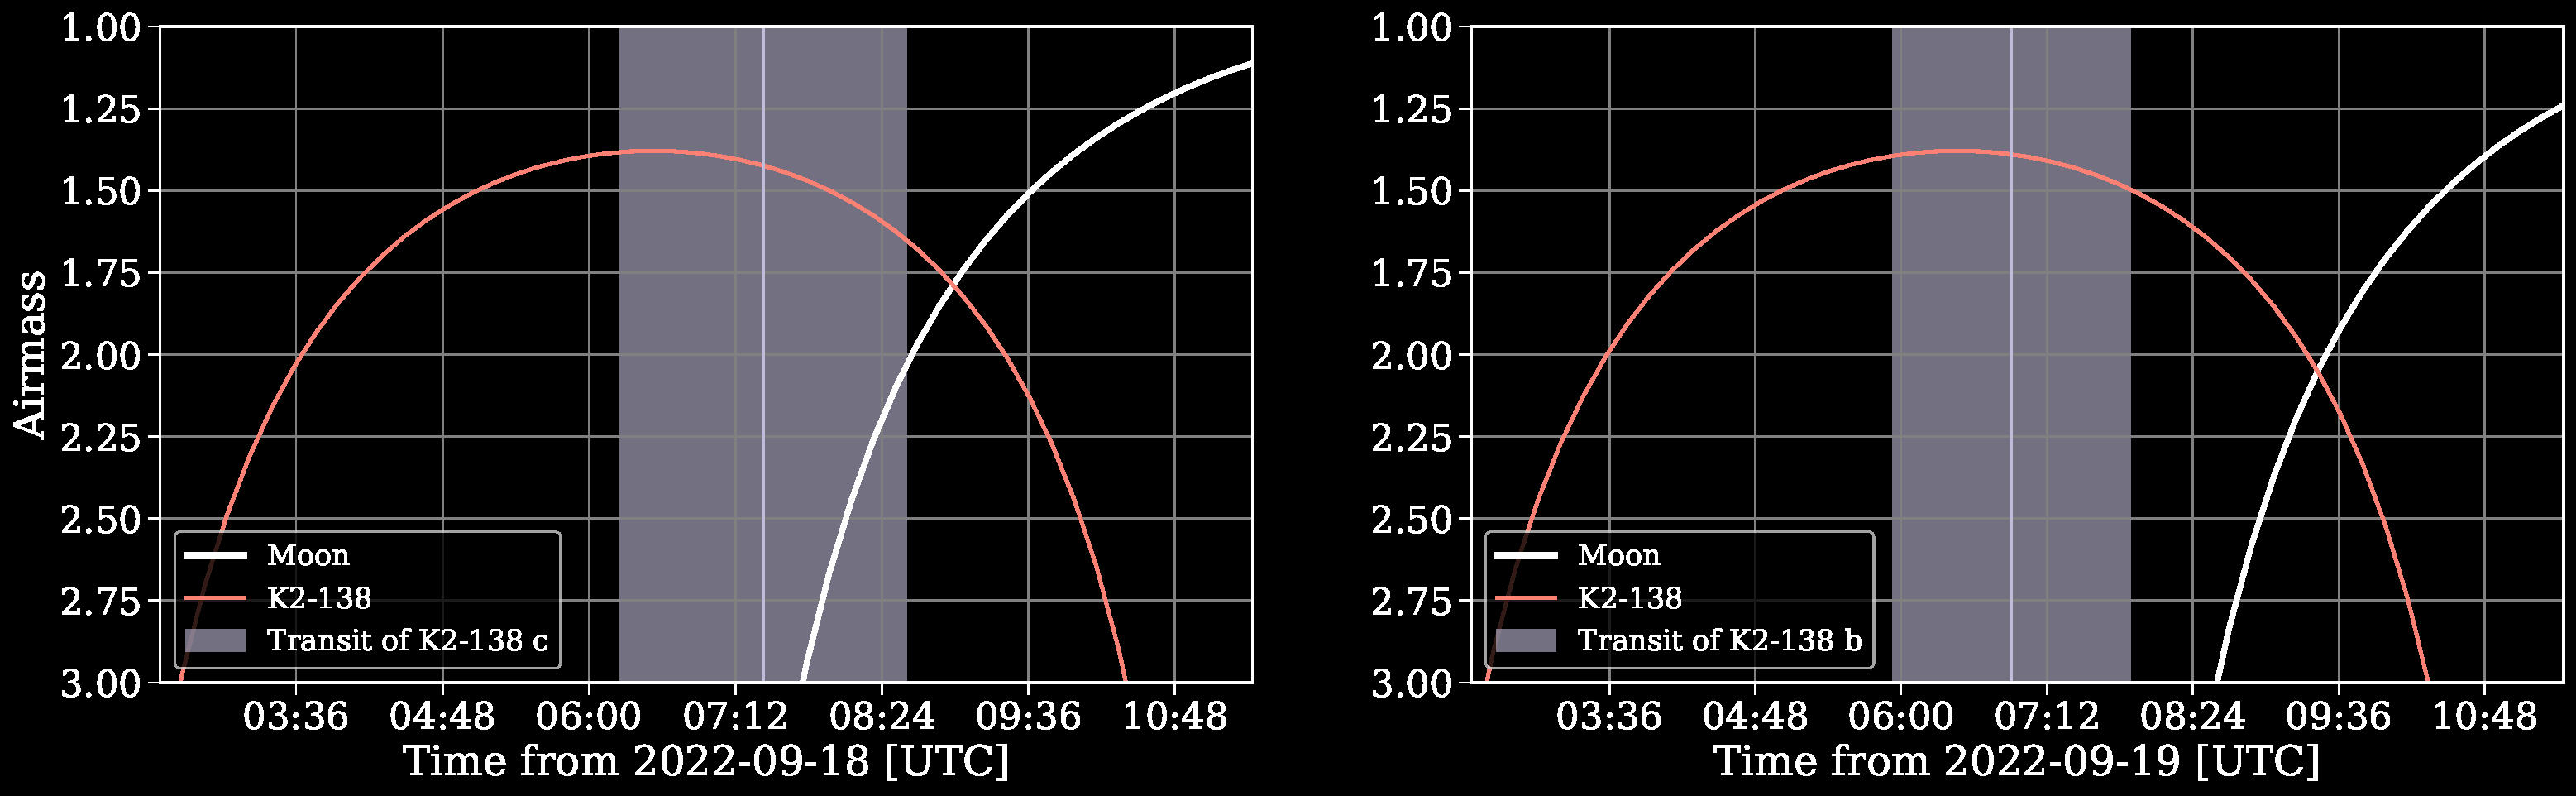
\includegraphics[width=\columnwidth]{observable_transits.pdf}
    \caption{}
\end{figure}


\bibliographystyle{aasjournal}
\bibliography{proposal}{}

\end{document}